%!TEX program = xelatex
\PassOptionsToPackage{full}{textcomp}
\documentclass[lang=en,11pt,a4paper,citestyle =authoryear,nobib=true]{elegantpaper}

% 标题
\title{HW4 - STAT 701}
\author{Wells Guan}

% 本文档命令
\usepackage{array,url,stix}
\usepackage{tikz}
\usepackage{tikz-cd}
\usepackage{enumitem}
\usepackage{amsmath}
\usepackage{amssymb}
\usepackage{listings}
\usepackage{subfigure}
\usepackage{placeins}

\lstset{
    frame=single,
    columns=fullflexible,
    keepspaces=true,
    showstringspaces=false,
    breaklines=true,
    breakatwhitespace=false,
    basicstyle=\ttfamily\footnotesize,
    numbers=left,
    numberstyle=\tiny,
    numbersep=6pt
}
\newcommand{\ccr}[1]{\makecell{{\color{#1}\rule{1cm}{1cm}}}}
\newcommand{\code}[1]{\lstinline{#1}}
\newcommand{\prvd}{$\hfill \qedsymbol$}
\newcommand{\Z}{\mathbb{Z}}
\newcommand{\R}{\mathbb{R}}
\newcommand{\N}{\mathbb{N}}
\newcommand{\C}{\mathbb{C}}
\newcommand{\Q}{\mathbb{Q}}
\newcommand{\M}{\mathcal{M}}
\newcommand{\B}{\mathcal{B}}
\newcommand{\X}{\mathcal{X}}
\newcommand{\Hil}{\mathcal{H}}
\newcommand{\range}{\mathcal{R}}
\newcommand{\nul}{\mathcal{N}}

% 文档区
\begin{document}

\maketitle

\subsection*{Problem 1}
Tell me where you are with your project! Please treat this as an opportunity
to touch base and ask some questions, for example about data issues, code
difficulties, anything like that. I would also appreciate the demonstration
that you've started doing something for it.

\par\vspace{0.5em}\noindent\textbf{Sol.}\par
I chose Option 1, Ensemble Kalman Filtering for nonlinear data assimilation
and rolling forecasting. For the application I am starting with the
three-dimensional Lorenz system rather than the financial example.

I have set up the basic simulation and observation pipeline. The state
transition uses a fourth-order Runge--Kutta step with
$(\sigma,\rho,\beta)=(10,28,8/3)$. I use step size $0.01$ and take an
observation every five steps. The current observation model is
\[
y_t=Hx_t+v_t,\qquad H=(1,0,0),\quad v_t\sim N(0,1),
\]
so that only one of the three coordinates is observed. I also included
small process noise with $Q=0.01I_3$ per observation interval. These are
initial experimental settings, not parameters estimated from real data.

The code currently generates a synthetic latent trajectory and noisy
observations, initializes an ensemble of size 40, propagates it through
the nonlinear dynamics, constructs the sample covariance, and checks one
stochastic EnKF update. For forecast ensemble members $x_t^{f,(i)}$,
the basic update I implemented is
\[
K_t=P_{xy,t}(P_{yy,t}+R)^{-1},\qquad
x_t^{a,(i)}=x_t^{f,(i)}+K_t\{y_t+v_t^{(i)}-Hx_t^{f,(i)}\}.
\]
I checked the array dimensions, finite values, and the symmetry and
nonnegative definiteness of the sample covariance. The preliminary
simulation below is only a check of the data-generation setup; it is not
a claim about filtering or forecasting performance.
\begin{figure}[htbp]\centering
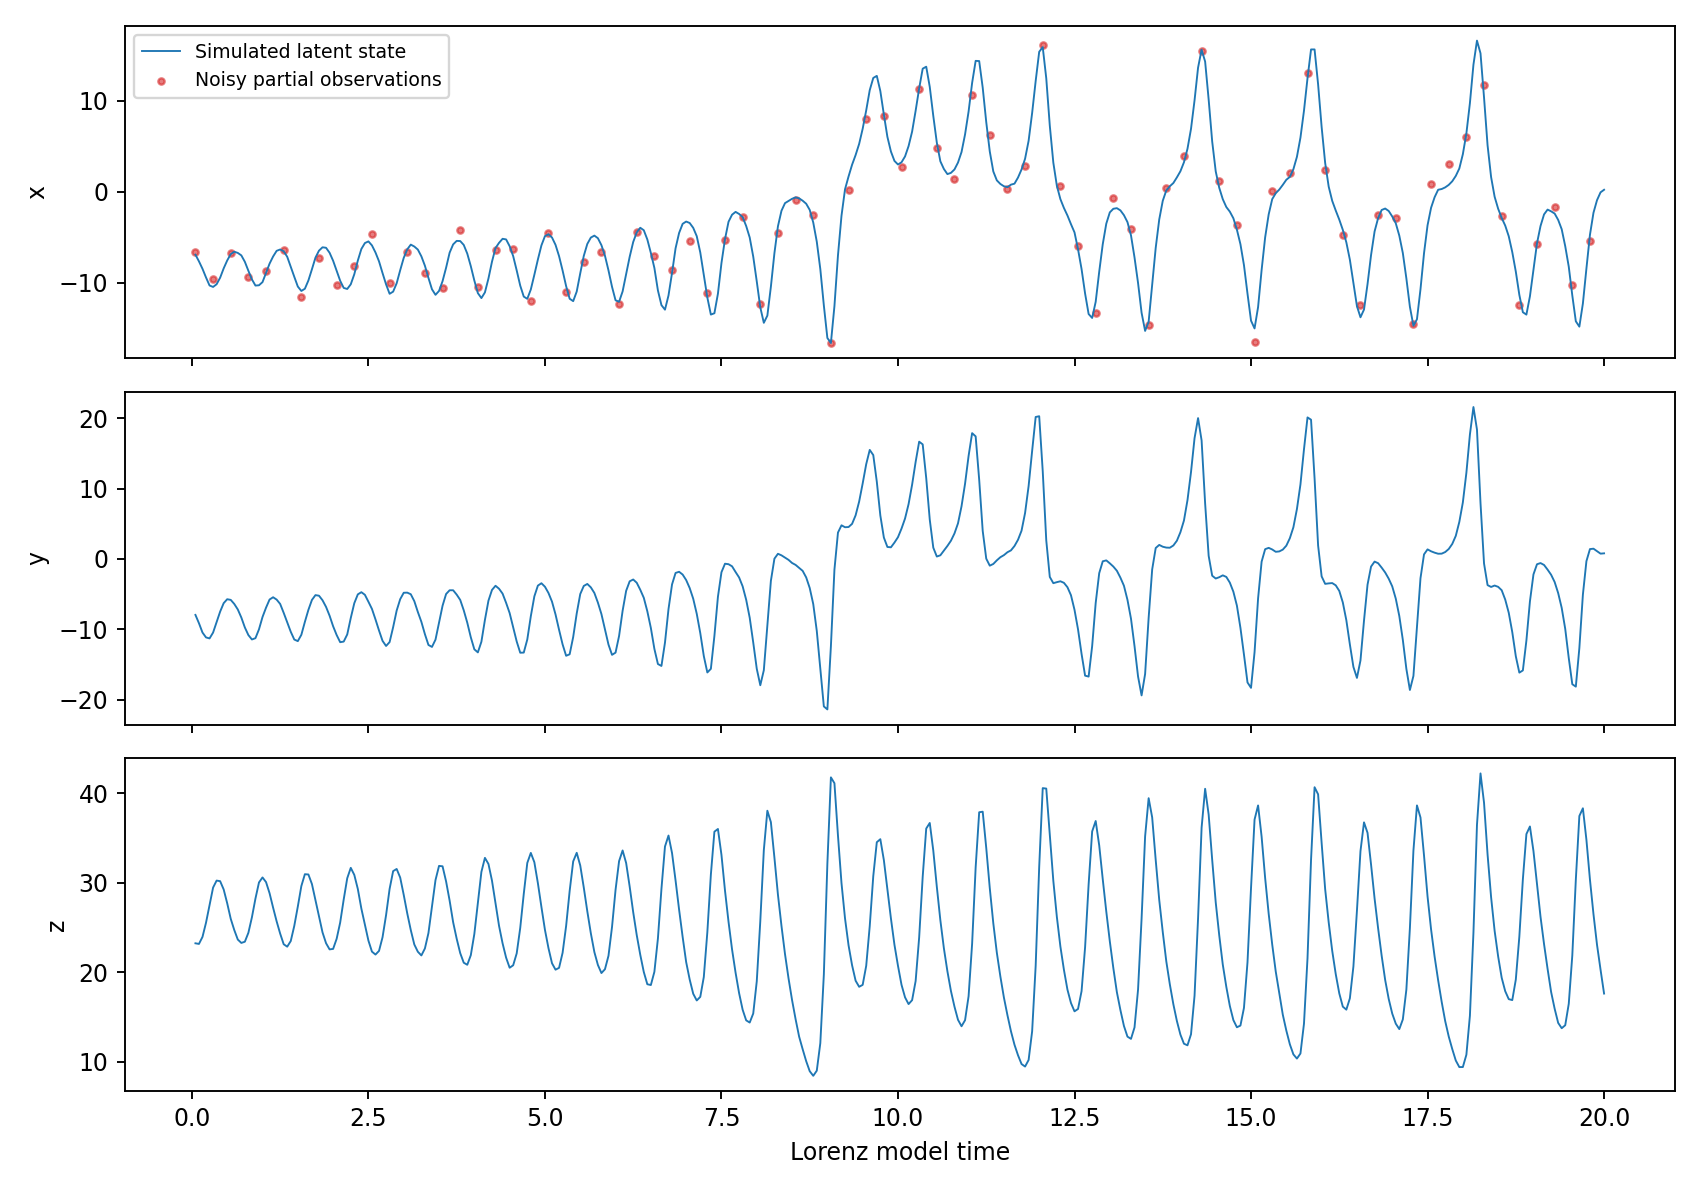
\includegraphics[width=0.85\linewidth]{png/project_setup.png}
\caption{Initial Lorenz simulation with noisy observations of the first
coordinate. The other two state coordinates are unobserved.}
\end{figure}

My next step is to run the full sequential filter and compare rolling
forecasts with a persistence baseline, without using future observations
in the updates. I plan to compare ensemble sizes $20,40,80,160$, summarize
RMSE and ensemble CRPS, and then examine whether covariance inflation
reduces divergence. I have not completed those experiments yet.
I would like to ask whether observing only the first coordinate is a
reasonable starting point, and what forecast horizons would give a useful
comparison before all methods lose skill because of the chaotic dynamics.

\vspace{1em}

\subsection*{Problem 2}
Fast forward in time: you are a professional time series specialist (which
I know you all will be), and somebody hands you a dataset that you don't
know the structure of (on canvas as \texttt{mystery\_data.csv}, and please
assume unit daily timesteps). They want two things: predictions for the
next year (365 future points), and confidence intervals for those predictions.
You notice a strong oscillatory component in the data, and you choose to
try and compare two models:
\[
\begin{aligned}
X_t&=\mu+\sum_{k=1}^{K}A_k\cos(\omega_k t)+B_k\sin(\omega_k t)+Y_t,
\qquad\text{and}\\
X_t&=\mu+Y_t,
\end{aligned}
\]
where $Y_t$ is a mean-zero stationary time series in both settings (but
maybe not the same one for each!).
\begin{enumerate}[label=\arabic*.,leftmargin=*]
\item Pick a stationary time series model for each $Y_t$, and fit the data
(including picking $K$ and frequencies $\{\omega_k\}_{k=1}^{K}$!) using any
of the tools we've discussed in class thus far. Look at as many diagonistics
as you can think of. For example (but you don't necessarily have to do all
of these things): negative log-likelihoods at the MLE, parameter values,
simulations from the fitted model, conditional simulations (which I claim
you know how to do if you're a little clever!), and whatever else seems
appropriate and useful to you. Based on those summaries, which model do
you prefer?

\par\vspace{0.5em}\noindent\textbf{Sol.}\par
I use Gaussian AR models for the stationary part in both settings. Write
\[
Y_t=\sum_{j=1}^{p}\phi_jY_{t-j}+Z_t,\qquad
Z_t\overset{\mathrm{i.i.d.}}{\sim}N(0,\sigma_Z^2),
\]
where $\phi(z)=1-\sum_{j=1}^{p}\phi_jz^j$ has no zeroes in $|z|\le1$.
For the first model I use
\[
m_H(t)=\mu+\sum_{k=1}^{K}\{A_k\cos(2\pi f_kt)+B_k\sin(2\pi f_kt)\},
\]
and for the second one $m_S(t)=\mu$. Here $f_k$ is in cycles per day and
$\omega_k=2\pi f_k$. The AR orders and innovation variances can differ
between the two models. In particular an AR(2) with conjugate roots can
represent stochastic oscillation without putting a sinusoid in the mean.

The supplied CSV has no header and contains $n=10000$ finite observations.
I read all 10000 values without treating the first observation as a column name.

For a given frequency set, I fit the regression coefficients, AR coefficients,
and innovation variance by the exact stationary Gaussian likelihood. If
$r=\mathbf X-\mathbf m$ and $\Gamma$ is the AR covariance matrix, the
negative log-likelihood is
\[
-\ell=\frac12\{n\log(2\pi)+\log\det\Gamma+r^\top\Gamma^{-1}r\}.
\]
I evaluate this likelihood by whitening the first $p$ observations with
their stationary covariance and the remaining observations with the AR
innovation filter. For each AR parameter vector, the mean coefficients
and innovation variance are profiled out. I use stationary parameterizations
and both Yule--Walker and nested lower-order starting values. I check the
resulting likelihood against the stationary state-space likelihood.
The models therefore use all observations on the same scale.

I search $p=0,\ldots,12$ for each model. For the harmonic mean I take up to
three separated periodogram peaks, consider $K=1,2,3$ when available,
and refine their frequencies by profile least squares within $0.49/n$ of
the selected Fourier frequencies. The likelihood fit is conditional on
these selected frequencies; I do not claim a joint global MLE over
frequencies. I select the converged candidate with the smallest
\[
\mathrm{BIC}=-2\ell+(p+3K+2)\log n.
\]
There are $2K+1$ mean coefficients, $K$ frequencies, $p$ AR coefficients,
and one innovation variance. For the stationary-mean model, $K=0$.
This is a finite candidate comparison, not a proof that the selected
order or frequencies are the true ones.

I inspect the standardized one-step innovations, their ACF, normal Q--Q
plots, and Ljung--Box tests. The tests are descriptive because orders and
frequencies were selected from the data. I also draw from each fitted
model using a stationary Gaussian initial state for its AR component.
The simulations show whether the apparent oscillation looks like a
fixed phase or a random phase that slowly loses coherence. Failed
likelihood fits are excluded, and the selected fits must converge.

\IfFileExists{results/full_summary.tex}{\begin{center}\begin{tabular}{lrrrr}
Model & $K$ & $p$ & $-\ell$ & BIC\\\hline
harmonic & 1 & 2 & -25965.060 & -51865.648\\
stationary & 0 & 12 & -25695.754 & -51262.563\\
\end{tabular}\end{center}
\noindent\textbf{harmonic.} 
The fitted periods in days are $188.51$. 
The fitted parameters are listed in the order
\[\mu,A_1,B_1,\ldots,\phi_1,\ldots,\sigma_Z^2.\]
Their numerical values are
\[\begin{gathered}-0.014801,\ 1.0036,\ -1.2128,\ 1.9749,\ -0.98327,\ 0.00032488\end{gathered}\]
Innovation Ljung--Box $p$-values (lag: value) are 10: 0.05935, 20: 0.161, 40: 0.09522.\par
\noindent\textbf{stationary.} 
The fitted parameters are listed in the order
\[\mu,A_1,B_1,\ldots,\phi_1,\ldots,\sigma_Z^2.\]
Their numerical values are
\[\begin{gathered}-0.013869,\ 2.0267,\ -1.0345,\ 0.0054856,\ -0.013638,\ 0.031718\\-0.039969,\ 0.039947,\ -0.06232,\ 0.062747,\ -0.0048459,\ -0.068221\\0.054415,\ 0.00034283\end{gathered}\]
Innovation Ljung--Box $p$-values (lag: value) are 13: 0.002487, 20: 0.0001397, 40: 0.00181.\par
For this fitted candidate set, BIC favors the harmonic model. This is an in-sample comparison.\par}{
\par\noindent\textit{The Canvas data have not been supplied. The fitted
parameters, likelihood comparison, and numerical model preference cannot
yet be evaluated.}}
For these candidates, I prefer the harmonic model in sample. It uses one
period of about $188.51$ days and an AR(2) residual. Its innovation tests
at lags 10, 20 and 40 give $p$-values about $0.059$, $0.161$ and $0.095$.
The constant-mean AR fit still has significant innovation correlations,
and its selected order is at the upper search limit of 12. Thus I do not
regard that fit as fully adequate. A larger AR search or an ARMA model
could improve the stationary alternative, and this comparison does not
prove that the oscillation is truly deterministic. Negative values of
$-\ell$ are possible here because these are continuous densities and the
innovation variance is small.

\IfFileExists{png/data_overview.png}{
\begin{figure}[htbp]\centering
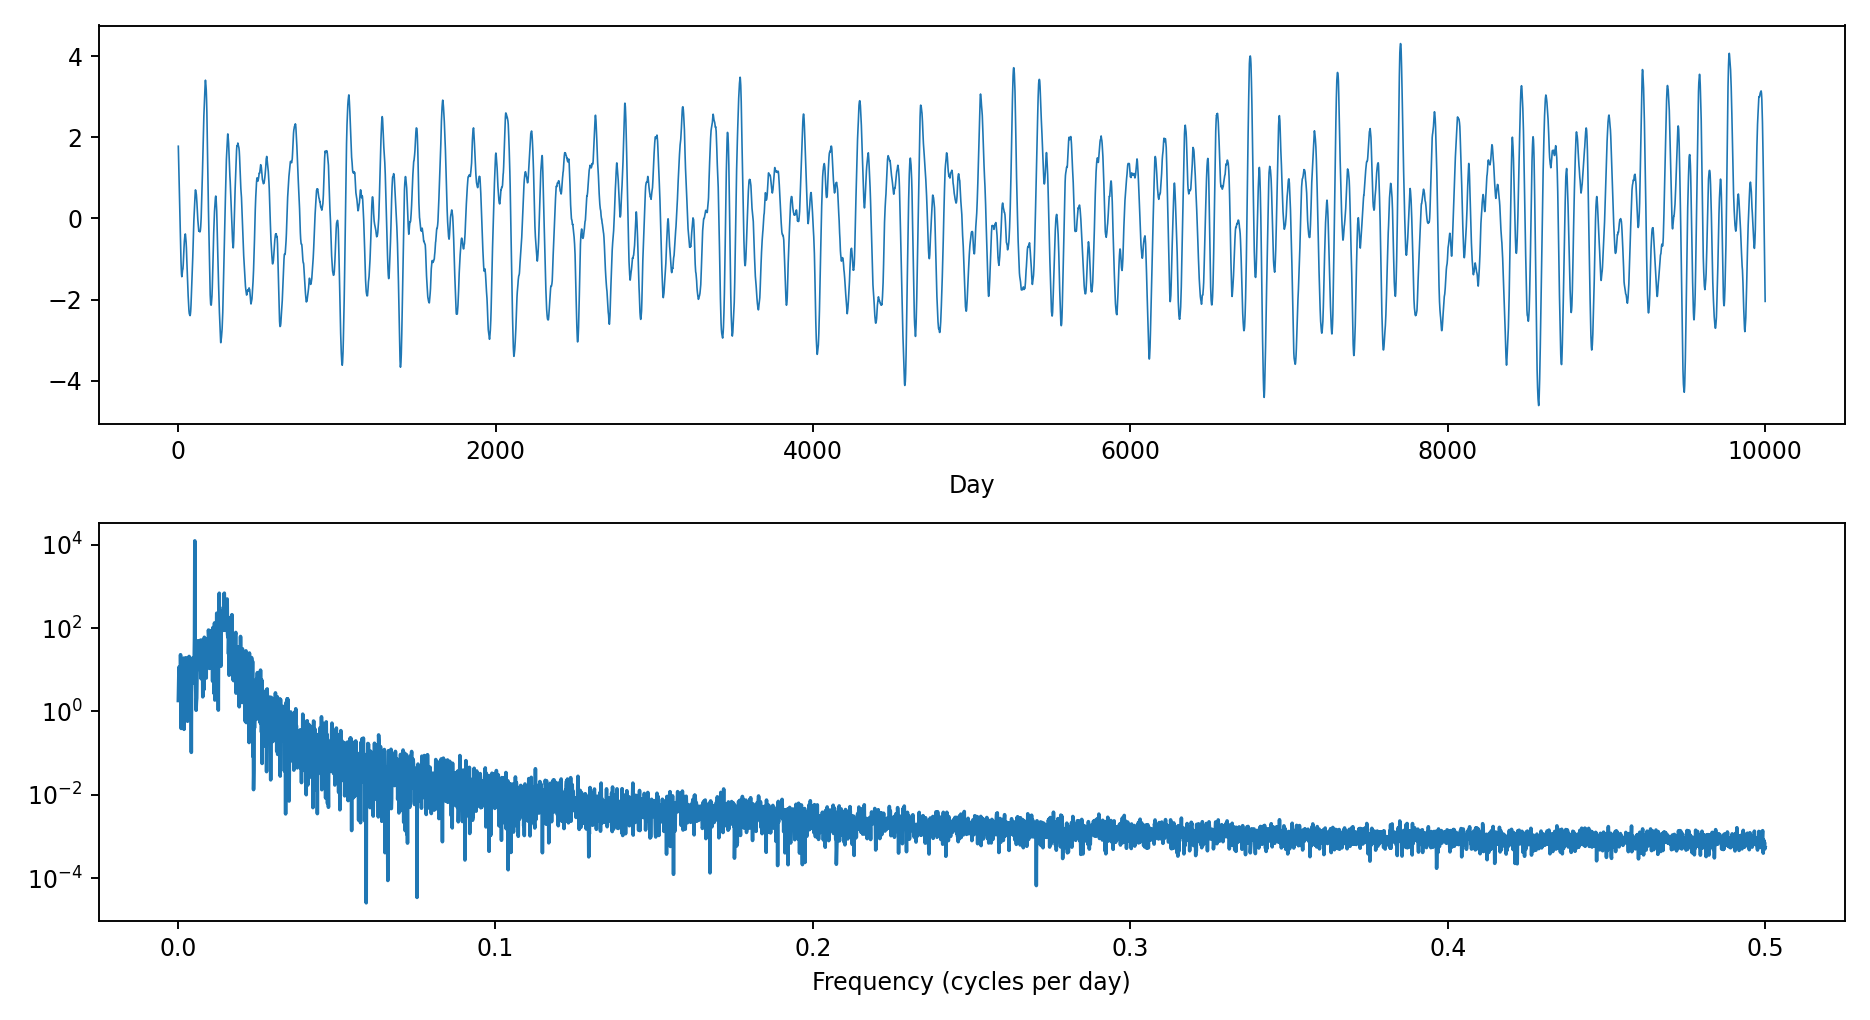
\includegraphics[width=0.92\linewidth]{png/data_overview.png}
\caption{The observed series and its periodogram.}\end{figure}}{}
\IfFileExists{png/full_diagnostics.png}{
\begin{figure}[htbp]\centering
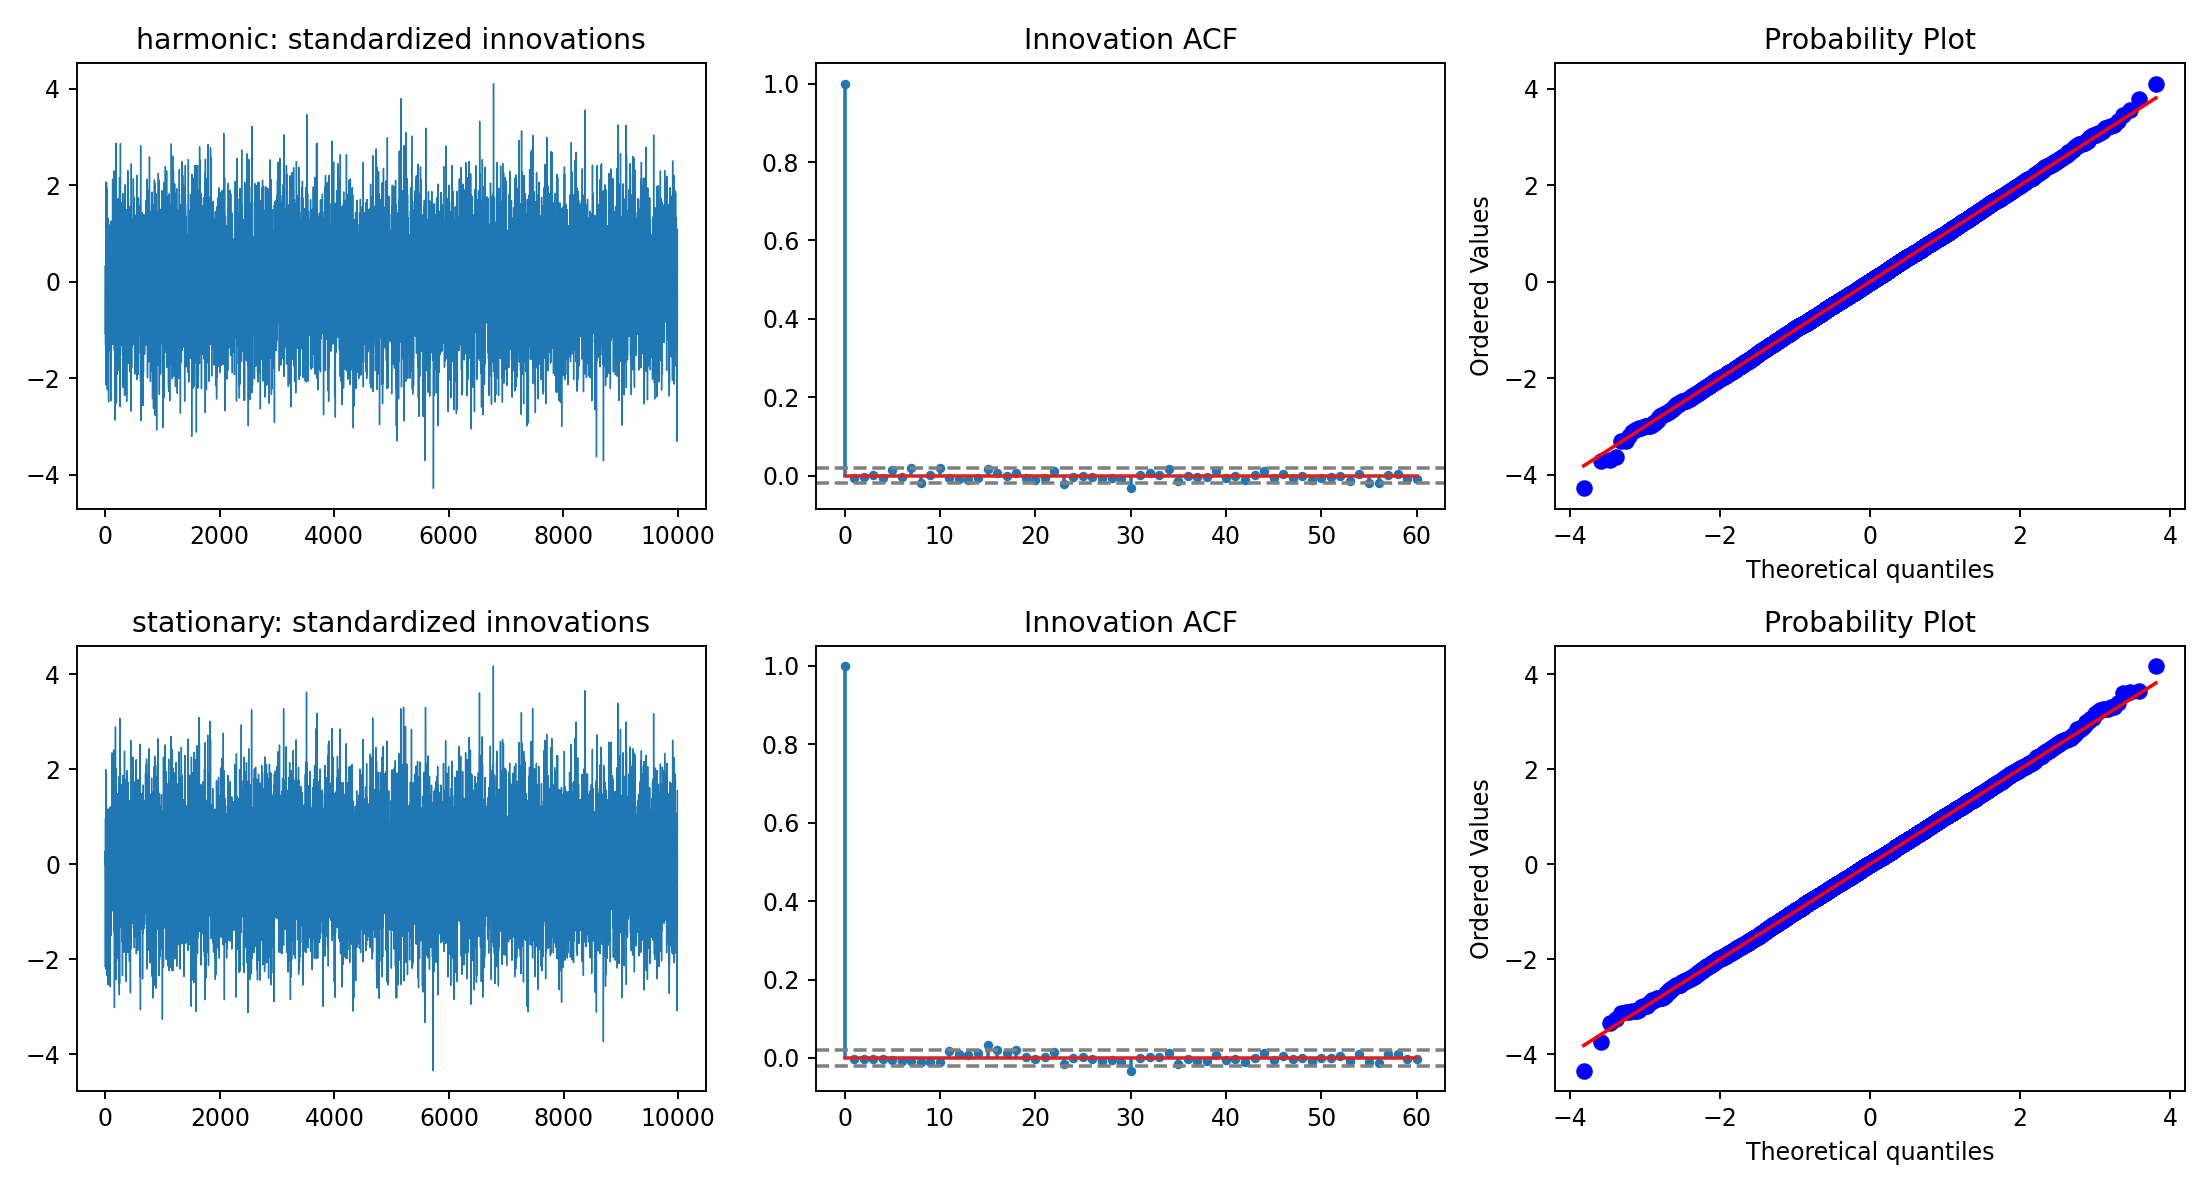
\includegraphics[width=0.98\linewidth]{png/full_diagnostics.png}
\caption{Full-data innovation diagnostics for the two fitted models.}\end{figure}}{}
\IfFileExists{png/full_simulations.png}{
\begin{figure}[htbp]\centering
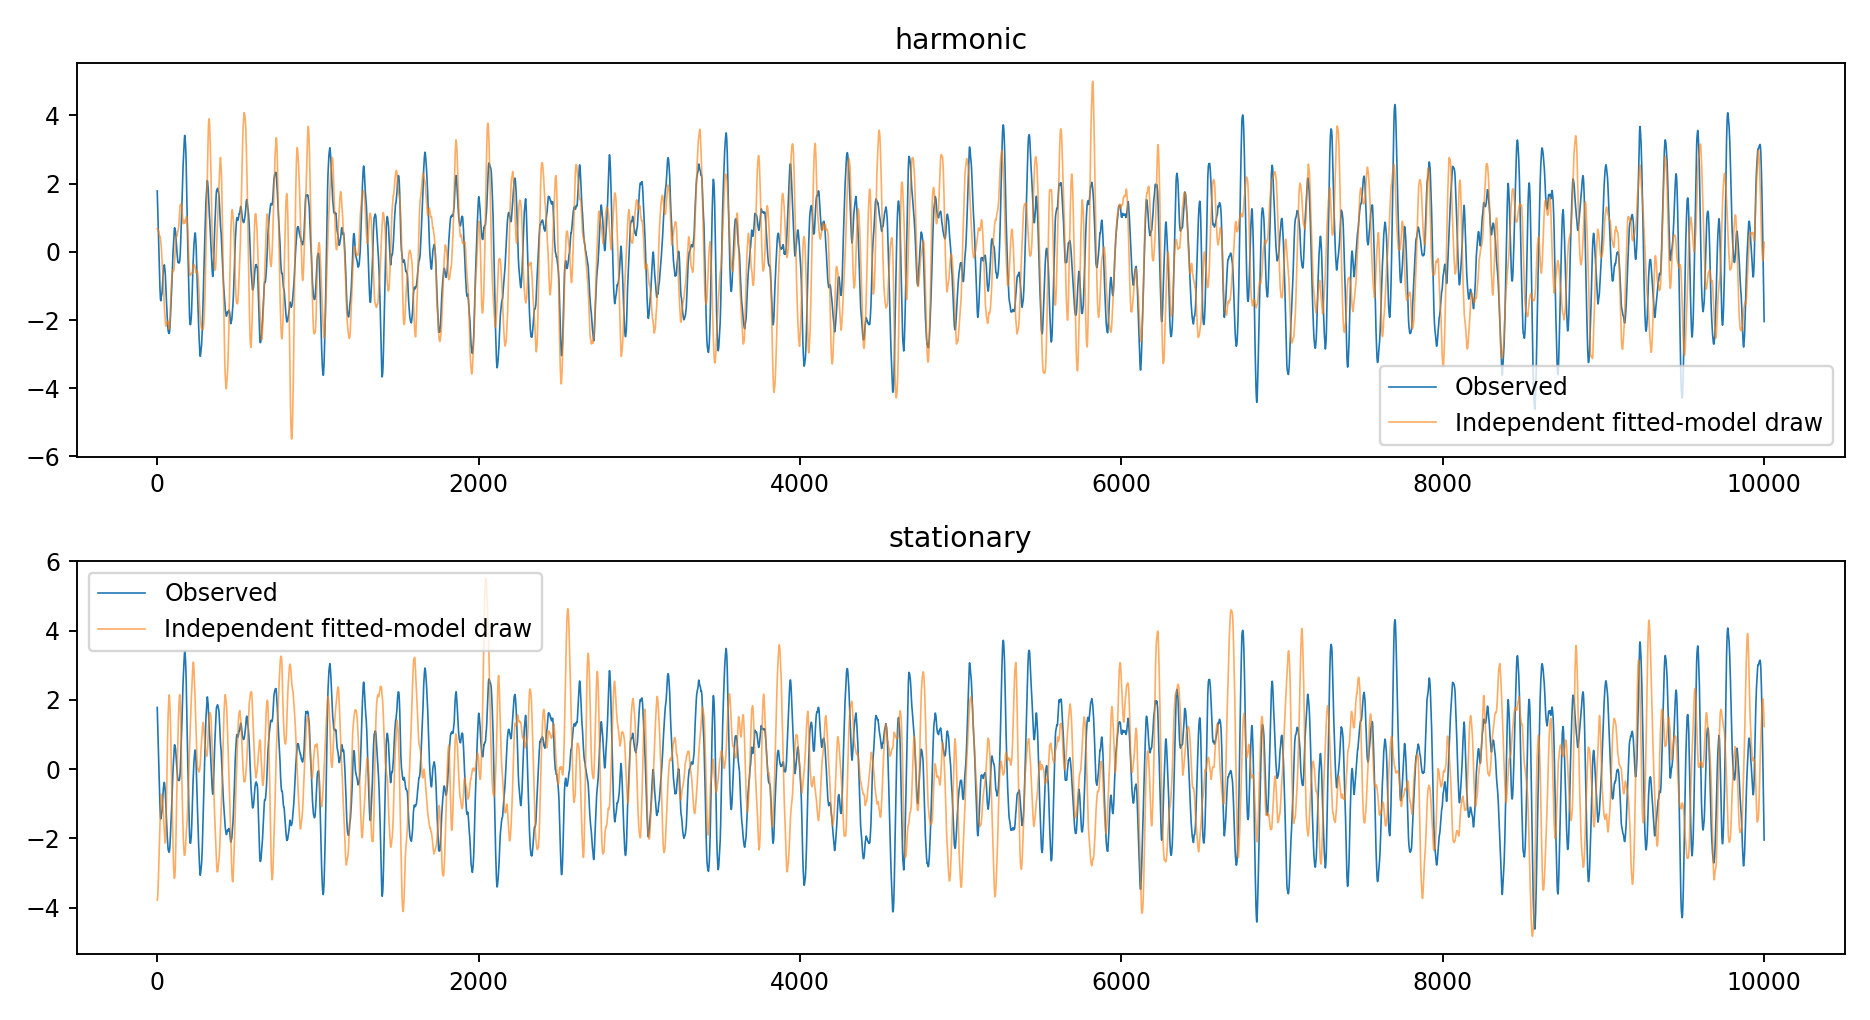
\includegraphics[width=0.95\linewidth]{png/full_simulations.png}
\caption{Observed data and independent draws from the fitted models.}\end{figure}}{}

\vspace{1em}

\newpage
\item Now compute your predictions and 95\% confidence intervals for them
via
\[
1.96\cdot\sqrt{V[X_{n+h}\mid X_1,\ldots,X_n]}.
\]
For each model, plot the predictions and uncertainties for them.
Which model do you prefer?

\par\vspace{0.5em}\noindent\textbf{Sol.}\par
For each fitted model, put $\mathbf m=(m(1),\ldots,m(n))^\top$,
$\Gamma_n=[\gamma(i-j)]_{i,j=1}^n$, and
$c_h=(\gamma(n+h-1),\ldots,\gamma(h))^\top$. By Gaussian conditioning,
\[
\widehat X_{n+h\mid n}=m(n+h)+c_h^\top\Gamma_n^{-1}(\mathbf X-\mathbf m),
\]
\[
v_h=V[X_{n+h}\mid\mathbf X]=\gamma(0)-c_h^\top\Gamma_n^{-1}c_h.
\]
The covariance is that of the stationary residual $Y_t$ for the specified
model. The interval is
$\widehat X_{n+h\mid n}\pm1.96\sqrt{v_h}$, $h=1,\ldots,365$.
It is a pointwise prediction interval, rather than a simultaneous band
or an interval for the conditional mean alone.

For the fitted AR model, the same calculation can be done without forming
$\Gamma_n$. Starting from the final $p$ residuals, use
\[
\widehat Y_{n+h\mid n}=\sum_{j=1}^{p}\phi_j\widehat Y_{n+h-j\mid n},
\quad \widehat Y_{t\mid n}=X_t-m(t)\quad(t\le n).
\]
If $\psi_0=1$ and
$\psi_j=\sum_{i=1}^{\min(p,j)}\phi_i\psi_{j-i}$, then
\[
\widehat X_{n+h\mid n}=m(n+h)+\widehat Y_{n+h\mid n},\qquad
v_h=\sigma_Z^2\sum_{j=0}^{h-1}\psi_j^2.
\]
The code checks these means and variances against the state-space forecasts.
I also obtain conditional simulations by adding future independent
$N(0,\sigma_Z^2)$ innovations to the AR recursion, starting from the same
observed residual history.

These intervals condition on fitted parameters and frequencies. They do
not include uncertainty from estimation or model selection, and actual
coverage may be lower than 95\%. In the harmonic model the mean oscillation
persists at long horizons; in the stationary-mean model the forecast
approaches $\mu$. Both residual prediction variances approach their own
stationary residual variances. The fixed sinusoid contributes no conditional
variance once its coefficients and frequency are treated as known.
Thus narrower intervals alone do not imply better forecasts.

Over the next 365 points, the harmonic forecast keeps the slow fitted
oscillation after the AR residual forecast has largely decayed. The
constant-mean forecast instead returns toward its fitted mean. I provisionally
prefer the harmonic forecast because its full-data diagnostics are better,
but the future observations are unavailable. The holdout experiment below
is the available forecasting check, rather than the width of the full-data
intervals by itself.

\IfFileExists{png/full_forecasts.png}{
\begin{figure}[htbp]\centering
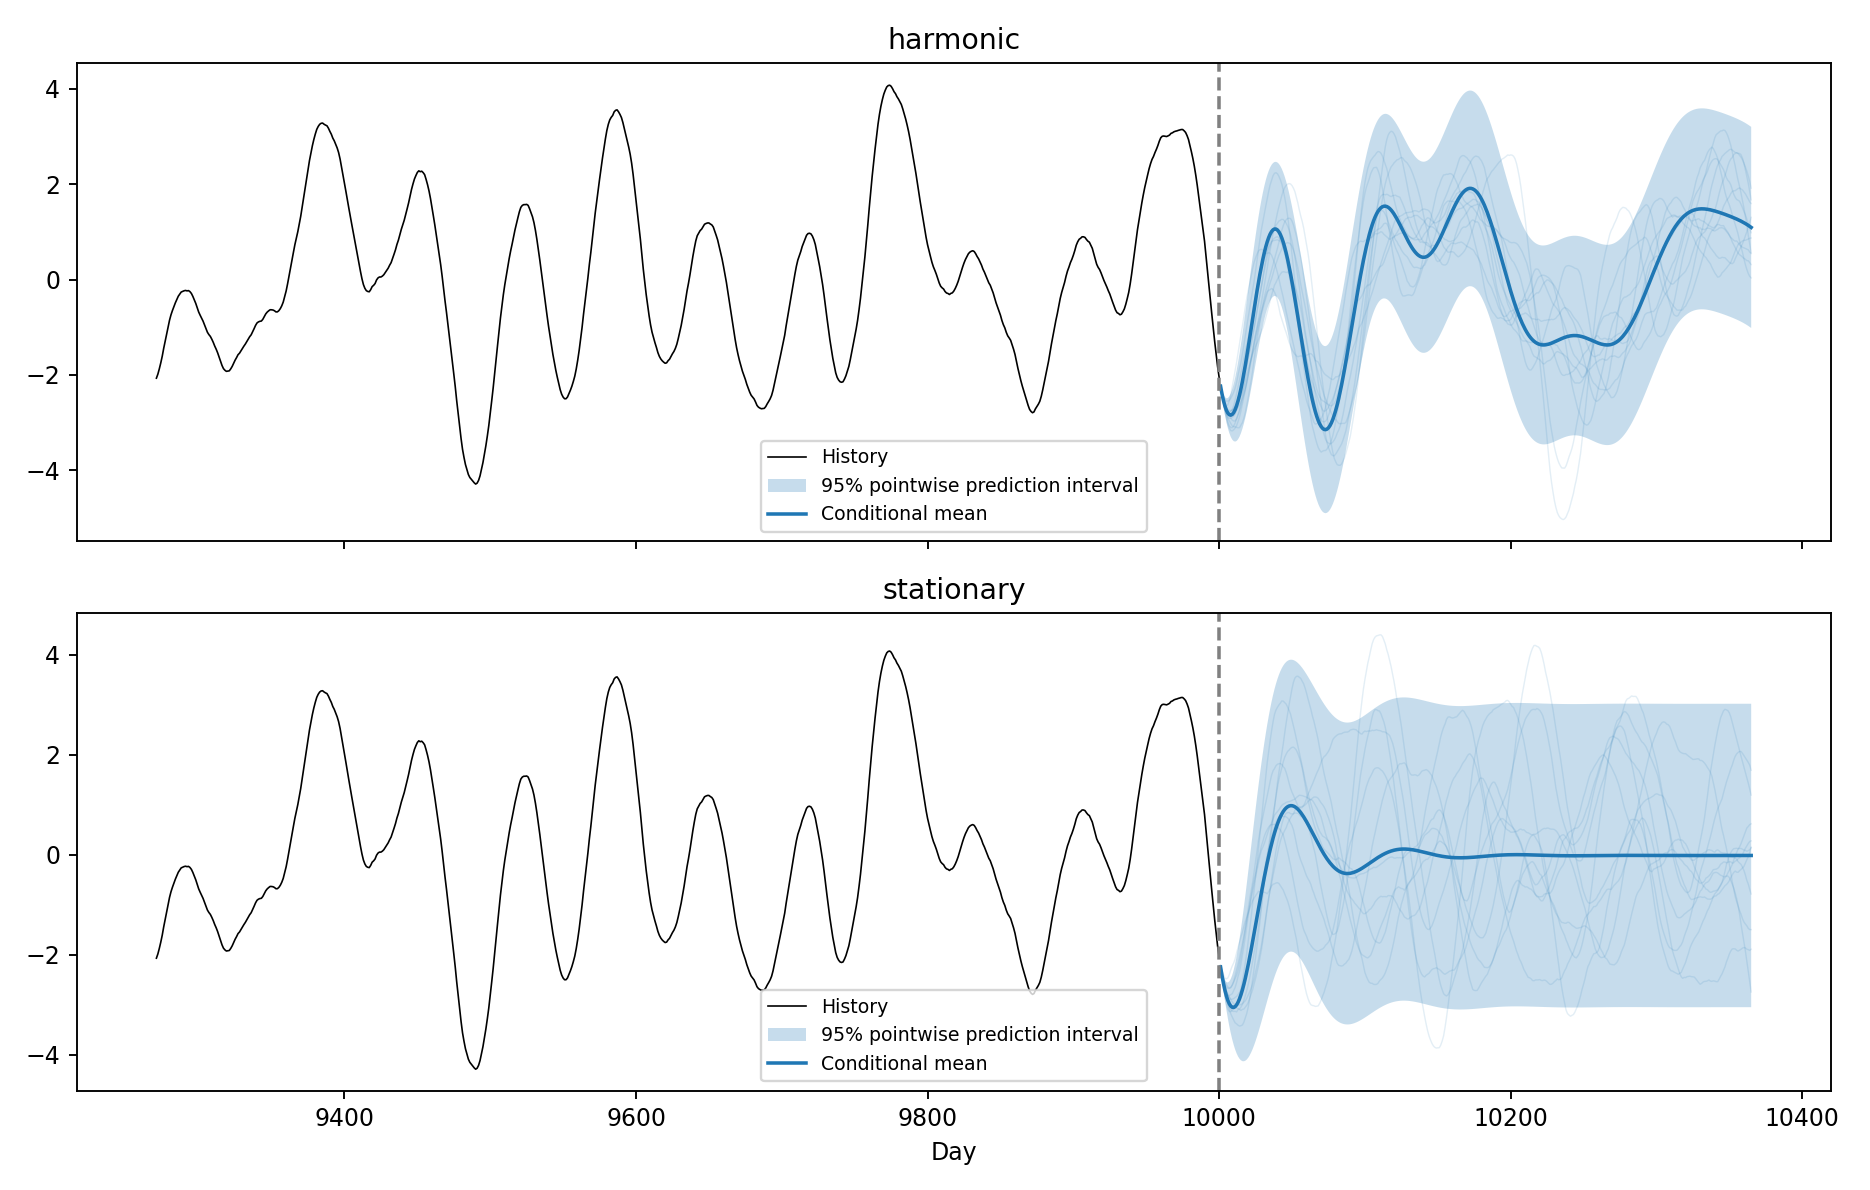
\includegraphics[width=0.98\linewidth]{png/full_forecasts.png}
\caption{Next-year forecasts, pointwise 95\% prediction intervals, and ten
conditional simulated paths for each full-data fit.}\end{figure}}{
\par\noindent\textit{The forecast plot and a data-based preference are
pending the supplied Canvas observations.}}

\vspace{1em}

\item Now repeat steps 1 and 2, but apply it to data points
$\{X_1,\ldots,X_{n-365}\}$, and then plot your predictions and intervals
with the true holdout data $\{X_{n-365},\ldots,X_n\}$.
Which model do you prefer?

\par\vspace{0.5em}\noindent\textbf{Sol.}\par
I use the last 365 observations as the holdout. There is an indexing
issue in the question: the displayed holdout contains 366 values
and shares an endpoint with the training set. I use
$\{X_1,\ldots,X_{n-365}\}$ for training and
$\{X_{n-364},\ldots,X_n\}$ for testing.

I repeat the entire order and frequency selection using only the training
sample, then forecast the next 365 values without updating from the holdout.
In particular, the full-data periodogram is not used to select frequencies
for this experiment. I compare RMSE, MAE, pointwise coverage, average
interval width, and the 95\% interval score. For a holdout value $x$ and
interval $[l,u]$, the score is
\[
\mathrm{IS}_{0.05}(l,u;x)=(u-l)+40(l-x)\mathbf1_{\{x<l\}}
+40(x-u)\mathbf1_{\{x>u\}}.
\]
It penalizes both wide intervals and missed observations, so a model does
not improve this score simply by making all intervals wider.

\IfFileExists{results/holdout_summary.tex}{\begin{center}\begin{tabular}{lrrrr}
Model & $K$ & $p$ & $-\ell$ & BIC\\\hline
harmonic & 1 & 2 & -25018.522 & -49972.832\\
stationary & 0 & 12 & -24758.227 & -49388.030\\
\end{tabular}\end{center}
\noindent\textbf{harmonic.} 
The fitted periods in days are $188.49$. 
The fitted parameters are listed in the order
\[\mu,A_1,B_1,\ldots,\phi_1,\ldots,\sigma_Z^2.\]
Their numerical values are
\[\begin{gathered}-0.018608,\ 1.0265,\ -1.1882,\ 1.9744,\ -0.98271,\ 0.00032479\end{gathered}\]
Innovation Ljung--Box $p$-values (lag: value) are 10: 0.06025, 20: 0.2446, 40: 0.1006.\par
\noindent\textbf{stationary.} 
The fitted parameters are listed in the order
\[\mu,A_1,B_1,\ldots,\phi_1,\ldots,\sigma_Z^2.\]
Their numerical values are
\[\begin{gathered}-0.012542,\ 2.0228,\ -1.0264,\ -0.00086408,\ -0.010404,\ 0.029887\\-0.04287,\ 0.048165,\ -0.064889,\ 0.059991,\ -0.0035431,\ -0.069934\\0.055587,\ 0.00034279\end{gathered}\]
Innovation Ljung--Box $p$-values (lag: value) are 13: 0.0009956, 20: 0.000129, 40: 0.001276.\par
For this fitted candidate set, BIC favors the harmonic model. This is an in-sample comparison.\par}{}
\IfFileExists{results/holdout_metrics.tex}{\begin{center}\begin{tabular}{lrrrrr}
Model & RMSE & MAE & Coverage & Width & Interval score\\\hline
harmonic & 1.1689 & 0.9424 & 0.9123 & 3.7509 & 5.2947\\
stationary & 1.8139 & 1.4347 & 0.8877 & 5.7106 & 7.7797\\
\end{tabular}\end{center}
The harmonic model has the smaller holdout RMSE, and the harmonic model has the smaller interval score. 
I use the holdout results to assess forecasting; a single holdout year cannot establish that either model is the true mechanism.}{
\par\noindent\textit{Holdout errors, coverage and model preference require
the actual observations; no simulated data are substituted for them.}}
The harmonic fit gives RMSE $1.1689$ versus $1.8139$, and its mean interval
score is $5.2947$ versus $7.7797$. I therefore prefer it for this holdout year.
The empirical coverages are $91.23\%$ and $88.77\%$, both below $95\%$.
The harmonic intervals are narrower and have the better interval score,
but they are not perfectly calibrated. Estimation uncertainty, remaining
misspecification, and the particular held-out path may all matter. The
365 errors are dependent, so these coverages should not be interpreted as
365 independent Bernoulli trials.

\IfFileExists{png/holdout_forecasts.png}{
\begin{figure}[htbp]\centering
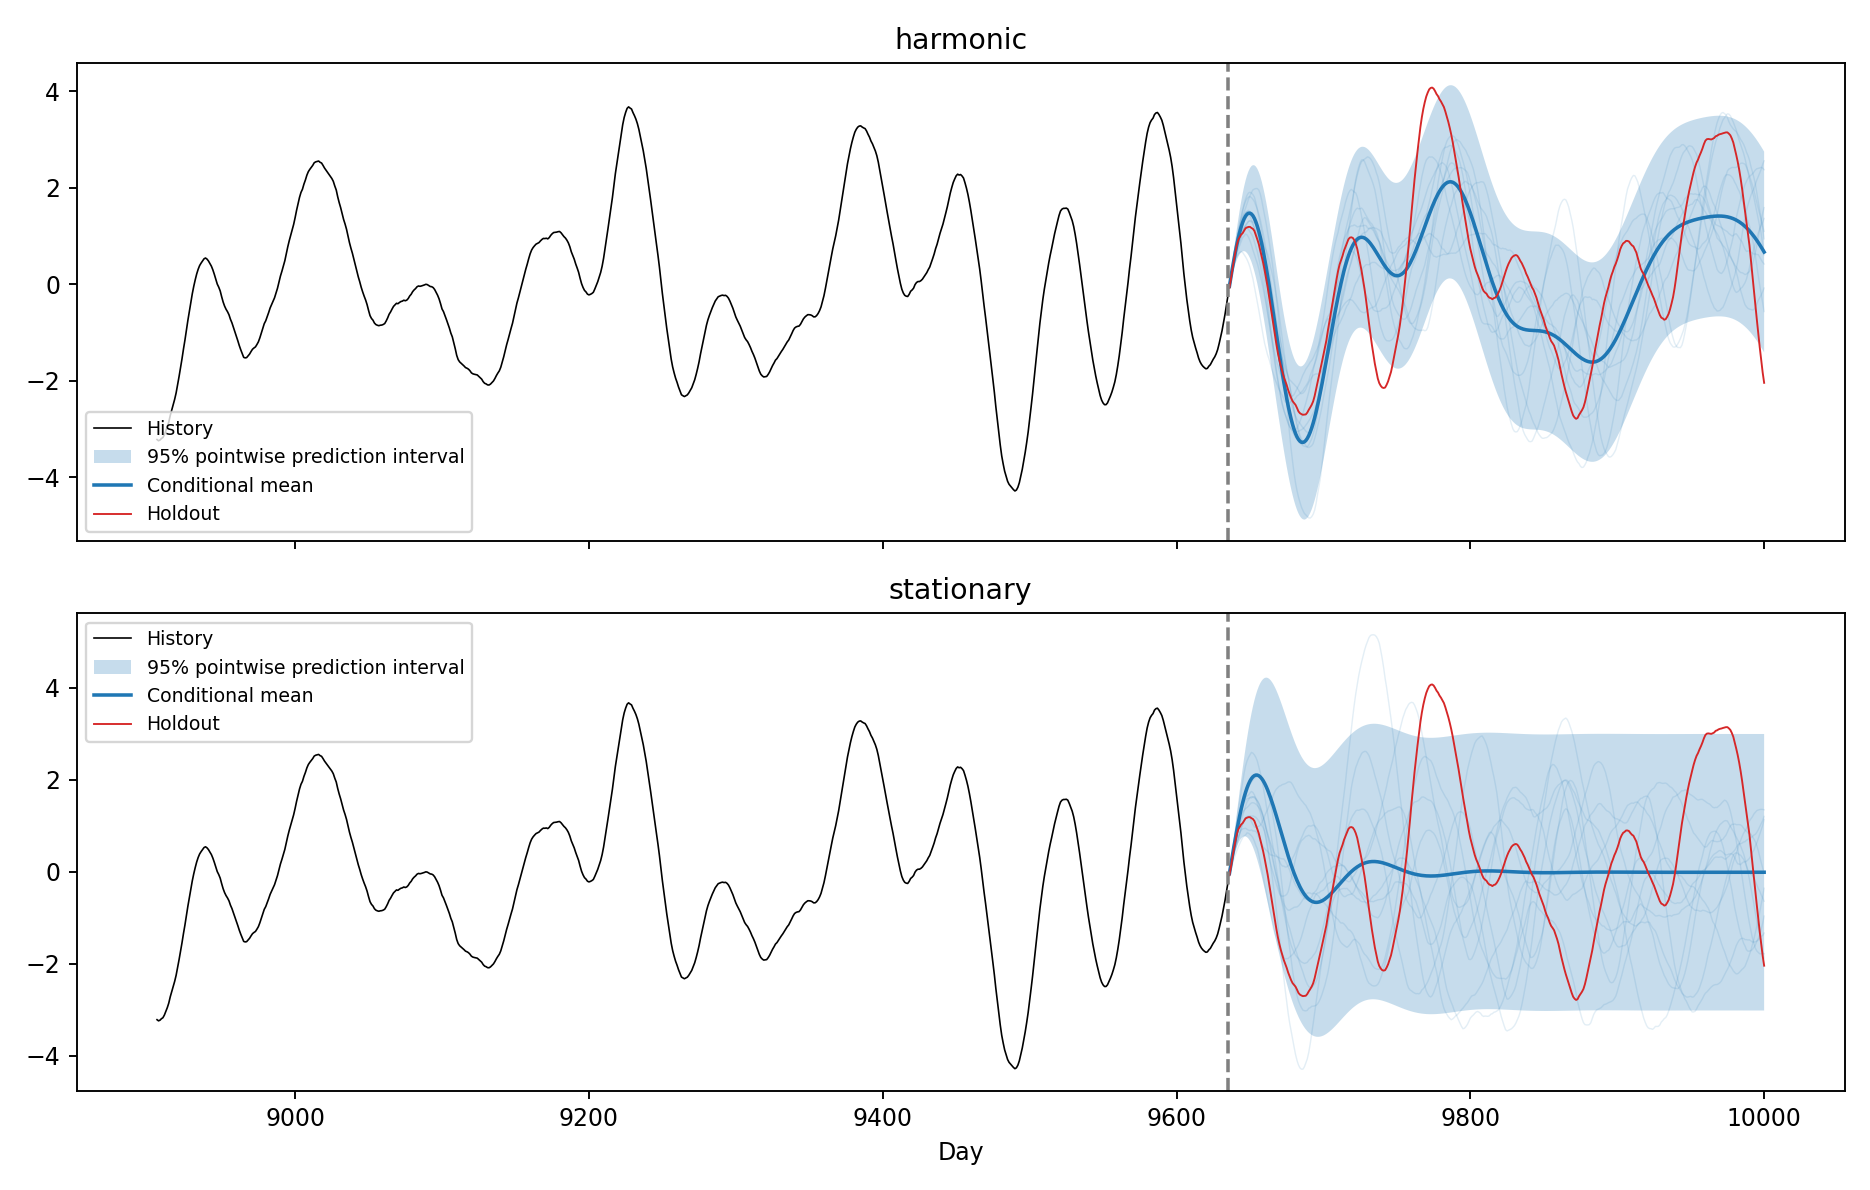
\includegraphics[width=0.98\linewidth]{png/holdout_forecasts.png}
\caption{Forecasts from the training sample, with the final 365 observations
shown in red. All model selection is repeated within training.}\end{figure}}{}
\IfFileExists{png/holdout_diagnostics.png}{
\begin{figure}[htbp]\centering
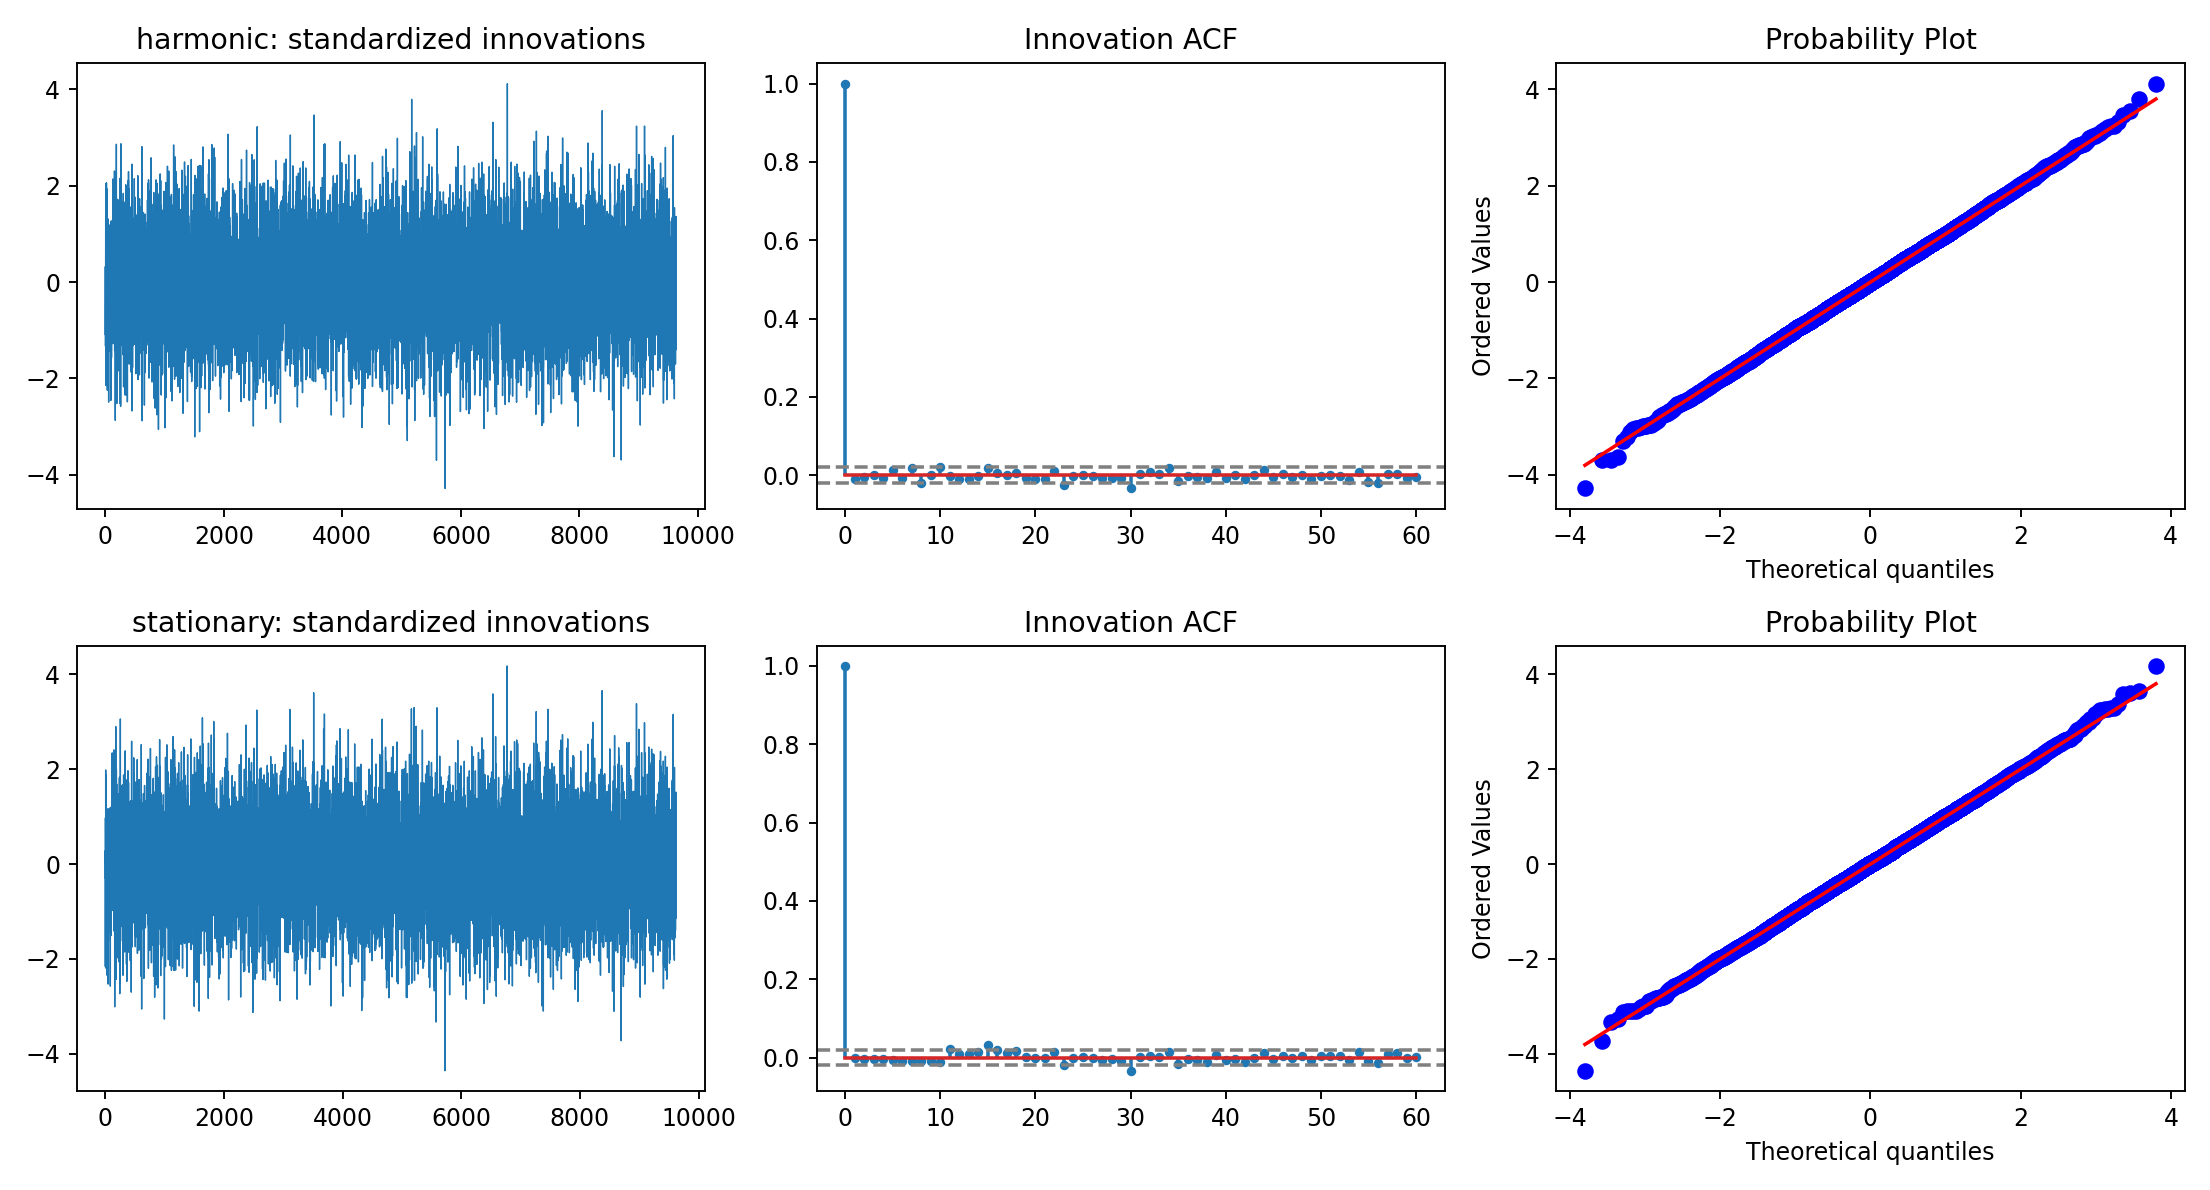
\includegraphics[width=0.98\linewidth]{png/holdout_diagnostics.png}
\caption{Innovation diagnostics for the training-only fits.}\end{figure}}{}

\vspace{1em}

\item Try to think of at least two examples in which the person who gave
you the data could offer additional context that would make you change
your preference.

\par\vspace{0.5em}\noindent\textbf{Sol.}\par
One example is an external clock. If the oscillation is caused by a
known periodic forcing, such as a controlled machine operating on a fixed
schedule, then a persistent harmonic mean is reasonable. The frequency
should be tied to that mechanism rather than only to a narrow peak in a
short record. I would be more willing to use the harmonic model in this case.

Another example is a randomly forced damped oscillator. A resonance can
produce a very sharp spectral peak even though its future phase is not
fixed. If the context is a natural system that is repeatedly perturbed,
I would put the oscillation in the covariance and prefer the stationary
model, provided its diagnostics are adequate. Its forecasts lose phase
information and return toward the mean, which is appropriate for this
mechanism.

Context can also invalidate both fits. A change in the operating schedule,
a sensor replacement, or a physical regime change during the forecast
year would make extrapolating either fitted stationary model questionable.
The same observed oscillation can therefore lead to different model
preferences depending on how the data were generated.

\vspace{1em}

\item A common practice in applied work is to model long-term non-stationary
trends using polynomial functions of time, $\mu(t)=\sum_{p=0}^{P}\beta_p t^p$,
rather than differencing or modeling long-memory in $Y_t$.
\begin{enumerate}[label=(\alph*),leftmargin=*]
\item Explain how fitting a polynomial mean trend to a process whose ACF
decays very slowly without oscillating suffers from similar mathematical
pathologies (regarding point forecasts, $h\to\infty$ behavior, and
conditional variances) as fitting pure sinusoids to a stochastic oscillatory
system like this one.

\par\vspace{0.5em}\noindent\textbf{Sol.}\par
Consider a stationary process with mean $\mu$ and $\gamma(h)\to0$
very slowly. Its finite-history Gaussian predictor is
\[
\mu+c_h^\top\Gamma_n^{-1}(\mathbf X-\mu\mathbf1),
\qquad v_h=\gamma(0)-c_h^\top\Gamma_n^{-1}c_h.
\]
For fixed $n$, $c_h\to0$ as $h\to\infty$, so the predictor tends to
$\mu$ and its conditional variance tends to $\gamma(0)$. Long memory can
make this convergence slow; it does not make a particular observed trend
persist forever.

If I fit the slowly varying realization with a deterministic polynomial
$m(t)=\sum_{p=0}^{P}\beta_pt^p$ and a short-memory residual, the forecast
instead approaches $m(n+h)$ as the residual forecast dies away. For
$P\ge1$ and a nonzero leading coefficient, its magnitude grows without
bound as $h\to\infty$. Treating the fitted polynomial as known also removes
its variation from the conditional variance: the reported variance tends
only to the fitted residual variance. If the polynomial has absorbed
low-frequency random variation, this can give misleadingly small
uncertainties, although a smaller variance is not guaranteed for every fit.

The same issue occurs with a deterministic sinusoid fitted to stochastic
oscillation. The sinusoid need not diverge, but it keeps its fitted amplitude
and phase forever. A stationary stochastic oscillator with decaying
covariance eventually loses that predictability. In both cases the model
has assigned a random feature of the observed path to a deterministic mean,
so its long-horizon forecast can be wrong even if the in-sample fit is good.

There is also parameter uncertainty. Write
$d(t)=(1,t,\ldots,t^P)^\top$. An approximate additional mean-estimation
variance is
\[
d(n+h)^\top\operatorname{Cov}(\widehat\beta)d(n+h).
\]
It can grow at rate $h^{2P}$ and is absent from the plug-in residual interval.
For sinusoidal regression, frequency error can likewise cause increasing
phase uncertainty. Including parameter uncertainty helps describe that
risk, but it does not repair a deterministic mean that is physically wrong.

\vspace{1em}

\item Describe a scenario where a global polynomial trend is scientifically
appropriate, versus one where that variation belongs in the covariance
function.

\par\vspace{0.5em}\noindent\textbf{Sol.}\par
A polynomial mean is reasonable if a physical mechanism specifies a
common trajectory over the time range of interest. For example, the
position of a body under known constant acceleration has a quadratic
mean trajectory; repeated measurements fluctuate around that trajectory.
The degree and the forecast range then have a scientific justification.
Even here I would not extrapolate past the time when the assumed force
law or experimental setup changes.

By contrast, the slowly varying part of a persistent environmental record
may be random: different realizations need not rise and fall at the same
times. I would place that variation in a long-memory covariance rather
than one global polynomial mean. If the trend is genuinely stochastic
and nonstationary, a nonstationary state model is needed.

\vspace{1em}
\end{enumerate}
\end{enumerate}

\FloatBarrier
\clearpage
\appendix
\section{Python code}
The following script fits both candidate families, produces diagnostics and
simulations, and repeats selection within the training sample for the holdout
experiment. The scripts contain no comments. Data belong in \texttt{data/},
figures in \texttt{png/}, and numerical summaries in \texttt{results/}.
The supplied Canvas observations are used for Problem 2. The synthetic
Lorenz observations are used only for the project setup in Problem 1.
\subsection{Project setup for Problem 1}
\lstinputlisting[language=Python,basicstyle=\ttfamily\scriptsize]{code/project_setup.py}
\clearpage
\subsection{Problem 2}
\lstinputlisting[language=Python,basicstyle=\ttfamily\scriptsize]{code/problem2.py}

\end{document}
